\documentclass[12pt]{article}


% Overall formatting
\sloppy
\let\cleardoublepage\clearpage % do not force chapters to start on odd pages


% Graphics
\usepackage{graphicx}
\DeclareGraphicsExtensions{.png,.pdf,.jpg}
\graphicspath{{Figures/}}


\usepackage[a4paper, total={16cm,25cm}]{geometry}



% Tables
\newlength{\mytabskip}   
\setlength{\mytabskip}{-1.5ex}
\newcommand{\tabrule}{\rule[\mytabskip]{0ex}{0ex}}
\usepackage{tabularx}
%\usepackage{longtable}


% bibliography stuff 
\usepackage{natbib}
\bibliographystyle{kluwer} 


\newcommand{\unit}[1]{\ensuremath{\mathrm{#1}}}
\newcommand{\degree}{\ensuremath{\mathrm{^\circ}}}

%\newcommand{\FIXME}[1]{{\sffamily \bfseries #1}}
\newcommand{\FIXME}[1]{{\sffamily {\bfseries \textcolor{red}{FIXME:} #1}}}


\hyphenation{EUMETSAT}
\hyphenation{Metop}



\begin{document}


\thispagestyle{empty}
\noindent
\textbf{\Large Study to support the definition of Arctic Weather \vspace{1mm}\\
Satellite (AWS) high frequency channels} \vspace{8mm}\\
{\bf Patrick Eriksson, Inderpreet Kaur and Simon Pfreundschuh}\\
Department of Space, Earth and Environment\\
Chalmers University of Technology\\
SE-412\,96, Gothenburg, Sweden\vspace{10mm}

\section*{Summary}
%
To be written \dots



\setcounter{tocdepth}{1} 
\tableofcontents


\newpage
\setcounter{page}{1}

\section{Introduction}
%
\subsection{Background}
The Arctic Weather Satellite (AWS) is a small platform carrying a single
radiometer package. This instrument is an across-track scanning microwave
radiometer. The exact channel configuration of AWS is not yet set. The main
issue for this report is that AWS will have channels at 183\,GHz, but also one
or several channels a higher frequencies. A number of channels around 325\,GHz
was considered as the main option before AWS became an ESA/EUMETSAT mission,
but it has now also been suggested to have a single channel at 229\,GHz. This
suggestion is based on MWS (MicroWave Sounder), one of the instruments onboard
the next generation of Metop satellites. The 229\,GHz was added to MWS as an
help for performing cloud screening of 183\,GHz data
\citep{rekha2012potential}. For comparison, it can be mentioned that ICI (Ice
Cloud Imager), another new Metop sensor, will include 325\,GHz channels.

\subsection{Aim}
%
To support the selection between 229 and 325\,GHz channels for AWS, this report
investigates the possibility to use the later range in forming 183\,GHz data of
``clear-sky'' character. That is, following \citet{rekha2012potential}, the
assumption, is that the 183\,GHz data will be used in an system not yet
capable of doing ``all -sky'' assimilation.

In \citet{rekha2012potential} the task was defined to screen out observations
having a cloud impact exceeding 4\,K at 183$\pm$7\,GHz. Their final suggestion
for screening does not involve data from any other channel than 229\,GHz, but
requires radiative transfer calculations (as a ``B-O test'' is made). Only 
screening of 183$\pm$7\,GHz was discussed.

In this report, the task is defined in a somewhat different manner. The aim is
not just to estimate the cloud impact, but also to investigate to which degree
the cloud impact can be removed, i.e.\ to make a cloud correction. Further, in
this report only schemes that can be based directly on AWS data will be
considered and versions involving ``B-O tests'' are left for possible future
studies. On the other hand, cloud correction of all AWS 183\,GHz channels are
investigated. Another important difference is that our simulations aim to be a
random sample of real situations, while the simulations of
\citet{rekha2012potential} have a strong over-representation of cloudy
cases.



\subsection{Comparison to \citet{rekha2012potential}}
\label{sec:rekha}
%
Results from \citet{rekha2012potential} will be used as reference. They did not
suggest specific settings of their algorithm. The main consideration of the
scheme is a threshold value. We assume below 6\,K for
this value, as it used most frequently as example in
\citet{rekha2012potential}. According to their Table~3, this results in that
2.4\% of the ``cloudy'' cases are miss-classified as ``clear''. We assume that
these cases have a cloud impact of 4 to 8\,K (i.e.\ the screening is 100\%
successful for cloud impact above 8\,K). For a 6\,K threshold 41\% of the
``clear'' cases are classified as ``cloudy'' and a removed in the screening
process. 

The selected threshold value is towards the high side of the ones considered by 
\citet{rekha2012potential}. A lower value improves the removal of ``cloudy'' cases,
but the fraction of incorrectly removed ``clear'' cases increases quickly. For
example, a threshold of 3\,K decreases the miss-classification of ``cloudy''
cases to 0.6\%, but increases the miss-classification for ``clear'' cases to 77\%.
If 183$\pm$7\,GHz is classified as cloudy, we assume that also the data from
other 183\,GHz channels are rejected.



\section{Assumptions on AWS characteristics}
%
The assumption listed below are primarily taken for the Statement of Work
(SoW), complemented with information provided by Anders Emrich at Omnisys
(private communication, April 14 2020). The later data represent what Omnisys
considers to be technically feasible inside the budget of the project.

\subsection{Channel specifications}
%
The specifications of channels around 89, 166, 183 and 229\,GHz are assumed to
be fixed, with name, position and widths defined in Table~\ref{tab:fixed:chs}.
AWS channels 31 to 36 will be implemented as a single front-end, but are here
still considered as two ``bands'', denoted as 166 and 183\,GHz, to more easily
separate the channels in the text. 

For 325\,GHz, it will be assumed that channels can be placed between 0.75 and
8.0\,GHz in terms of intermediate frequency (IF), and that up to 4 channels
inside this range can be implemented. There should be some gap between these
channels, above 100\,-\,200\,MHz, to facilitate the technical implementation.
For comparison, Table~\ref{tab:fixed:chs} includes also the position of 
325\,GHz channels of ICI. As the ICI channels extend to 11\,GHz in IF, they will not
be considered for AWS but will be applied for demonstration and reference
purposes.

For simplicity, the frequency variation of all channel responses is assumed to
be rectangular. This selection shall not be interpreted as any opinion on the
optimal shape of these responses; a significant deviation from a rectangular
shape should be of no concern as long as the actual shape is well
characterised.

\begin{table}[!b]
  \begin{minipage}[b]{0.5\linewidth}
  \centering  
  \begin{tabular}[c]{c|c|c}
    Channel & Frequency   & Bandwidth \\
    name    & [GHz] &  [MHz] \\
    \hline
    AWS-21  & \phantom{0}89.000 & 4000\\
    AWS-31  & 165.500 & 2800\\
    AWS-32  & 176.311 & 2000\\
    AWS-33  & 178.811 & 2000\\
    AWS-34  & 180.311 & 1000\\
    AWS-35  & 181.511 & 1000\\
    AWS-36  & 182.311 & \phantom{0}500\\
    AWS-4X  & 229.000 & 2000\\
    \hline
  \end{tabular}
  \end{minipage}%
  \begin{minipage}[b]{0.5\linewidth}
  \centering  
  \begin{tabular}[c]{c|c|c}
    Channel & Frequency   & Bandwidth \\
    name    & [GHz] &  [MHz] \\
    \hline
    ICI-5  & 325.15$\pm$9.50 & 3000\\
    ICI-6  & 325.15$\pm$3.50 & 2400\\
    ICI-7  & 325.15$\pm$1.50 & 1600\\
    \hline
  \end{tabular}
  \end{minipage}  
  \caption{Fixed channel position and widths. The left table covers channels of
    AWS, with values taken from SoW. Channels AWS-21 to AWS-36 are at this
    moment mandatory for AWS, while AWS-4X is so far tentative. The right table
    lists the values of some channels of ICI \citep{eriksson:towar:20}.}
  \label{tab:fixed:chs}
\end{table}


\subsection{Noise}
%
The nominal receiver noise temperature, $T_r$ of each band is listed in
Table~\ref{tab:trec}. The noise of data for individual channels is calculated
as
\begin{equation}
  \sigma^i = c \frac{T^i_r+T^i_a}{\sqrt{\Delta\!f^i\Delta t}}
  \label{eq:noise}
\end{equation}
where $\sigma^i$ is the noise standard deviation of channel $i$, $c$ is a
scaling factor (see below), $T^i_r$ is the receiver noise temperature of the
channel, $T^i_a$ is the antenna temperature of the channel, $\Delta\!f^i$ is
the bandwidth (in terms of IF) of channel and $\Delta t$ is the integration
time.

The factor $c$ is set to 1.2 to incorporate the additional noise caused by the
calibration process. The bandwidth applied is the one found in columns 3 of
Table~\ref{tab:fixed:chs}. The integration time is set to match an effective
15\,km resolution at 183\,GHz. This time was estimated to 3\,ms. 

\begin{table}[!bt]
  \centering
  \begin{tabular}[b]{c|ccccc}
    Band [GHz]   & 89 & 166 & 183 & 229 & 325 \\
    \hline
    $T_r$ [K]    & 390 & 650 & 650 & {\it 1000}  & 1200 \\
    \hline
  \end{tabular}
  \caption{Assumed receiver noise temperatures. The value for 229\,GHz is
    selected by us, remaining values are present assumptions at Omnisys.}
  \label{tab:trec}
\end{table}

\subsection{Various}
%
The AWS satellite is assumed to be at an altitude of 600\,km. Data were
generated for sensor viewing angles (the angle from nadir) from 0$^\circ$ to
45$^\circ$, in steps of 5$^\circ$.

The polarisation response of the bands is not yet determined and for simplicity
``quasi-horizontal'' (defined in same way as for e.g.\ MWS) is throughout
assumed. Antenna temperatures are obtained as:
\begin{equation}
  \label{eq:polrot}
  T_a = T_b^V\sin^2(\theta) + T_b^H\cos^2(\theta)
\end{equation}
where $T_b^V$/$T_b^H$ is the brightness temperature at vertical/horizontal
polarisation, respectively, and $\theta$ is the viewing angle (from nadir).



\section{Input data and software}

\subsection{Atmospheric scenarios}

\subsubsection{Fascod}
\label{sec:fascod}
%
The Fascod dataset \citep{anderson1986afgl} was used to represent different
climate zones in overview calculations. The dataset consists of profiles of
pressure, temperature and volume mixing ratio profiles of various atmospheric
gases. Five climatoligies were used: tropical (TRO), mid-latitude summer (MLS),
mid-latitude winter (MLW), sub-arctic summer (SAS), and sub-arctic winter
(SAW). No hydrometeors were included in simulations involving Fascod.


\subsubsection{Bulk profile database}
%
A database of atmospheric cases was created based on data from CloudSat and
ERA-Interim. The core idea of the approach is to use CloudSat reflectivities to
obtain as realistic vertical profiles of ice hydrometeors and rain as
possible. No external CloudSat retrievals are involved. Instead the CloudSat
reflectivities are mapped to properties for the passive simulations by assuming
a particle size distribution and a particle habit, together denoted as
the particle model. The process involves an inversion of the radar data, but as,
the same particle model is used for that inversion and to map ice water content
(IWC) and rain water content (RWC) to single scattering data when performing
the passive radiative transfer calculations, the impact of clouds on the
simulated AWS data is as realistic as possible. The thin clouds not detected by
CloudSat should not be of relevance for passive measurements frequencies
350\,GHz. Background data (temperature, humidity, 10\,m wind speed, \dots) were
taken from ERA-Interim, for the time and location of the CloudSat data. Liquid
water content (LWC) was taken from ERA-Interim, as CloudSat has no sensitivity
to the hydrometeor category.

This approach for generating atmospheric scenarios has been used by us since
\citet{rydberg:nonga:09}, and more recently in e.g.\
\citet{eriksson:towar:20} and \citet{barlakas:three:20}. It is also used in
\citet{ekelund:using:20}, where the approach is described more in detail. In
the cited articles, the sensor's footprint has been considered in varying
degree, as ``beam filling'' must be considered at high impact of hydrometeors.
As clear-sky and weak cloud interference are in focus in this study, and to
save calculation time, instead CloudSat data were averaged over 10\,km to form
the atmospheric cases and standard 1D radiative transfer calculations are
applied on each case (instead of applying an independent beam approximation
inside a 2D or 3D atmosphere as done in cited works).



\subsection{Radiative transfer simulations}
%
\subsubsection{ARTS}
%
All radiative transfer calculations are made by the Atmospheric Radiative
Transfer System (ARTS, \citet{eriksson:arts2:11,buehler:artst:18}), version
arts-2.3.????. Models and input used for absorption and hydrometeor properties
are described below. Ocean/water and land emissivities are taken from
TESSEM \citep{prigent2017sea} and TELSEM \citep{aires2011tool}, respectively.

Two calculations were performed for each atmospheric cases. One ''clear-sky''
where all hydrometeors contents were set to zero, and one ``all-sky'' where IWC
and RWC derived from CloudSat reflectivities and LWC from ERA-Interim were
included. Both sets of calculations were were made by ARTS's interface to the
RT4 solver \citep{evans1995microwavec}. This ``scattering solver'' was used
also for clear-sky, to avoid a possible bias between clear-sky and all-sky for
insignificant hydrometeor contents. RT4 handles the first two elements of the
Stokes vector, that were converted to brightness temperatures for H- and
V-polarisation.


\subsubsection{Absorption models}
%
The absorption of nitrogen is modelled following \citet{pwr:93}. Nitrogen has a
significant impact at least around 325\,GHz at dry conditions. Also oxygen
absorption follows \citet{pwr:93}. Oxygen is in this study mainly of concern
for the 94\,GHz CloudSat simulations. LWC was treated to be
purely absorbing, based on \citet{ellison2007permittivity}.

For water vapour the present settings in RTTOV are applied. That is, largely
MPM89 \citep{liebe:89} is followed, but some parameters for the 22 and 183\,GHz
transitions are replaced \citep{saunders2018update,turner2019amsutran}. A
smaller comparison to RTTOV has been made, that indicated an agreement better
than 0.1\,K in general. Deviations between 0.1 and 0.2\,K were found for some
channels at incidence angles above 40$^\circ$.


\subsubsection{Hydrometeor properties}
%
As mentioned above, LWC is taken from ERA-Interim and is assumed to be totally
absorbing. LWC is allowed to exist at temperatures below 0$^\circ$C, i.e.\
super-cooled liquid cloud droplets are present in the simulations. In the
mapping of CloudSat reflectivities to RWC and IWC a total separation between
liquid and ice phase is assumed. All scattering hydrometeors at temperatures
above 0$^\circ$C are assumed to be rain, and all below 0$^\circ$C are assumed
to be ice hydrometeors.

For RWC the particle size distribution of \citet{abel2012improved} is applied.
The PSD of IWC follows the basic formulation applied in DARDAR, using latest
parameter values (i.e.\ $\alpha$ and $\beta$) as given by
\citet{amt-12-2819-2019}. This PSD can be considered as a ``two moment''
scheme, but is here applied in a one moment manner by setting $N_0^*$ (as a
function of temperature) following Table~5 of \citet{delanoe2014normalized},
and letting the radar reflectivity set the remaining moment.

Single scattering data are taken from \citet{eriksson:agene:18}. For ice
hydrometeors, three habits are applied: Perpendicular 3-bullet rosette, Large
plate aggregate and Large column aggregate. In the two later cases, the
aggregates are complemented with single crystal data to also cover smaller
sizes. These data describe particles assumed to have a totally random
orientation. To apply oriented particles is much more computationally costly
and could not be accommodated inside the study.


\subsection{Validation of simulations}
\label{sec:validation}
%
Using the simulation setup described above, around 77000 cases were simulated
based on randomly selected CloudSat orbits during August 2015. The input data
were restricted between $60^{\degree}$S to $60^{\degree}$N. No differentiation
was made between the observations over water and land. 

\begin{figure}[p]
	\centering
	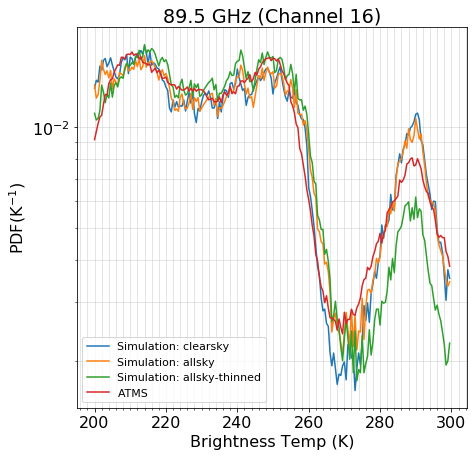
\includegraphics[height=60mm]{ATMS_C16_distribution}\hspace{5mm}% 
	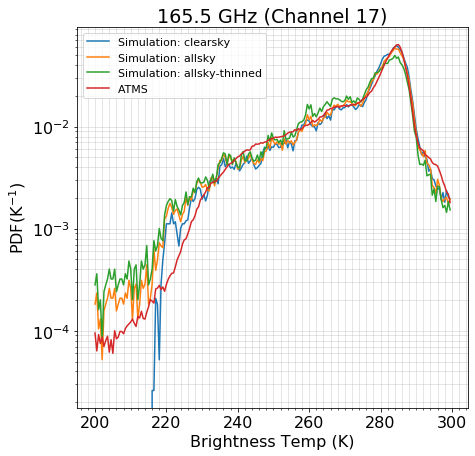
\includegraphics[height=60mm]{ATMS_C17_distribution}
	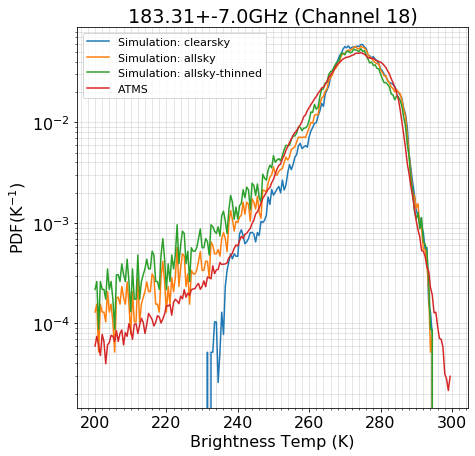
\includegraphics[height=60mm]{ATMS_C18_distribution}\hspace{5mm}% 
	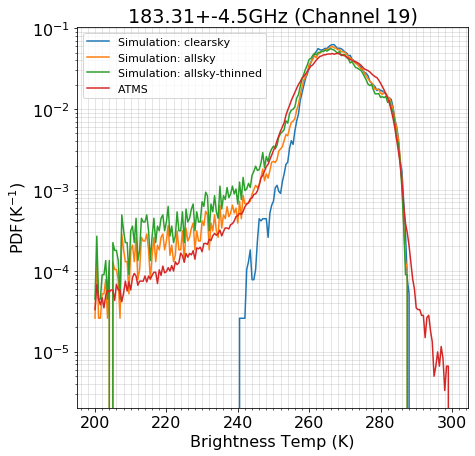
\includegraphics[height=60mm]{ATMS_C19_distribution}
	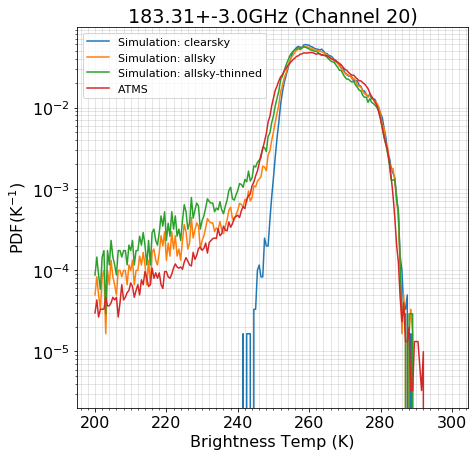
\includegraphics[height=60mm]{ATMS_C20_distribution}\hspace{5mm}% 
	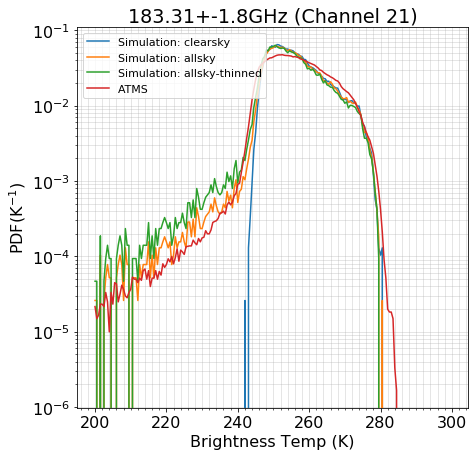
\includegraphics[height=60mm]{ATMS_C21_distribution}
	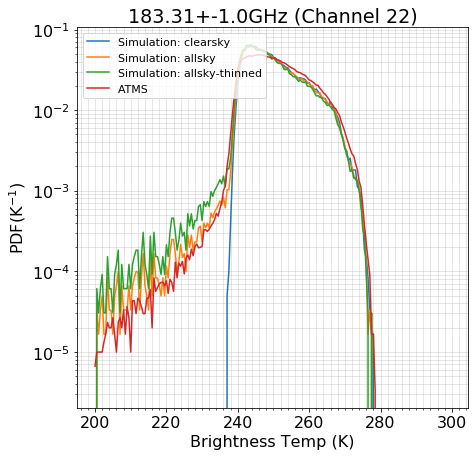
\includegraphics[height=60mm]{ATMS_C22_distribution}
	\caption{Probability distribution functions (PDFs) of simulated and
      observed ATMS channels brightness temperatures for channels 16 - 22 and
      nadir viewing angle. The data covers latitude range $60^{\degree}$S to
      $60^{\degree}$N. Both land and ocean measurements are considered and only
      daytime ATMS data are included. See further the text.}
	\label{fig:pdf:c16-22}
\end{figure}


A statistical comparison of the simulations to actual ATMS data, for channels
16-22 at nadir (zenith angle = $180^{\degree}$), is shown in
Fig.~\ref{fig:pdf:c16-22}. For the comparison, the daytime ATMS observations
were selected as CloudSat operates only during the day part of the orbit since
2011. For the channels around 183\,GHz, the ATMS characteristics are not fully
simulated. The ATMS channel widths are considered, but as AWS is only covering
the lower wing of the 183\,GHz transition the upper sideband of ATMS is not
included.

The overall agreement is good for channels. For 183 GHz channels (Channels
18-22), the simulations and observations have a good agreement for the part of
the PDFs matching clear-sky conditions (the main peak of the distribution),
albeit the simulations have a more sharp peak. This could either be caused by a
different geographical sampling of ATMS and CloudSat or to shortcomings in the
ERA-Interim input data. The fraction of cloudy observations is lower in ATMS in
comparison to simulations, for brightness temperatures below about 240\.K. This
is due to the fact that the antenna pattern is not considered in the
simulations.

In the intermediate region, the simulations have a lower occurrence rate. The
impact of hydrometeors should be somewhat higher in the upper sideband of ATMS,
which is not reflected in the simulations, but this is not sufficient to
explain the deviation. As this region is well covered in the simulations
reported in Fig.~7 of \citep{eriksson:towar:20}, the deviation of concern is
presumably also a consequence of the neglected antenna pattern. In this study,
this transitional region is of high interest. For this reason, the PDF for a
50\% random rejection of cases with an insignificant cloud impact is also
shown. This PDF gives a fair match in the intermediate region (but gives an
even higher overrepresentation at more strong cloud impacts). This smaller
dataset will be considered in parallel below, to ensure that no fraction of the
``cloudy'' cases is not underrepresentated in the results.





\section{Overview of the 183, 229 and 325\,GHz bands}
\label{sec:overview}
% 
The simulations in this section are based on five Fascod climate scenarios
(Sec.~\ref{sec:fascod}), and performed with a fixed sensor viewing angle of
25$^\circ$. No hydrometeors are included. For simpler interpretation of the
results, the reflectivity is set to have no frequency variation, i.e.\ the same
value is applied for all bands. The reflective is varied between 0 and 0.5.
In the figures covering transmissivities and Jacobians, the specifications
of ICI is applied for 325\,GHz channels (Table~\ref{tab:fixed:chs}).


\subsection{Clear-sky brightness temperatures}
%
Figure~\ref{fig:tb:r000} shows brightness temperatures over the three bands, for
a reflectivity of 0 (i.e.\ a blackbody surface). The figure takes into account
that the 183\,GHz channels of AWS are of single-sideband character, while for
229 and 325\,GHz averages of upper and lower sidebands are shown, plotted as
a function from the centre frequency on the lower side.

\begin{figure}[p]
  \centering
  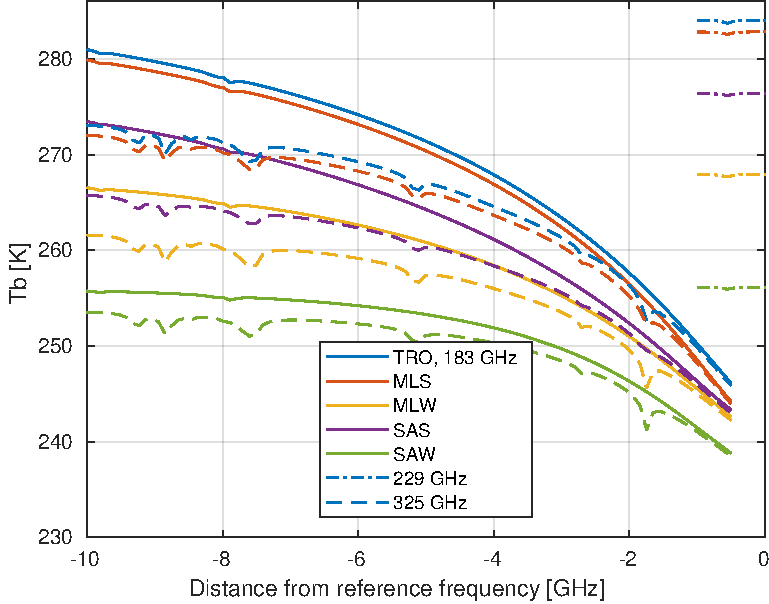
\includegraphics[width=0.75\textwidth]{fascod_tb_r000}
  \caption{Solid lines show brightness temperatures for the lower wing of the
    183.31\,GHz transition. Dashed lines represent double-sideband measurements
    around 325.15\,GHz, with the mean of upper and lower band shown on the low
    side. Dash-dotted lines represent double-sideband measurements around
    229.00\,GHz in the same manner, but only over the bandwidth of the
    potential channel. For all three bands, spectra for all five
    Fascod scenarios are included.}
  \label{fig:tb:r000}
\end{figure}
\begin{figure}[p]
  \centering
  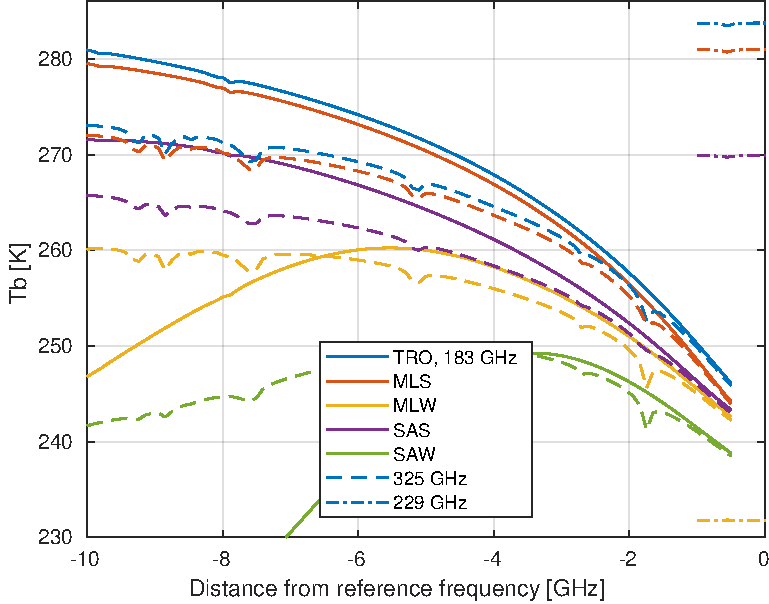
\includegraphics[width=0.75\textwidth]{fascod_tb_r050}
  \caption{Same as figure above, but with a surface reflectivity of 0.5.}
  \label{fig:tb:r050}
\end{figure}
\begin{figure}[p]
  \centering
  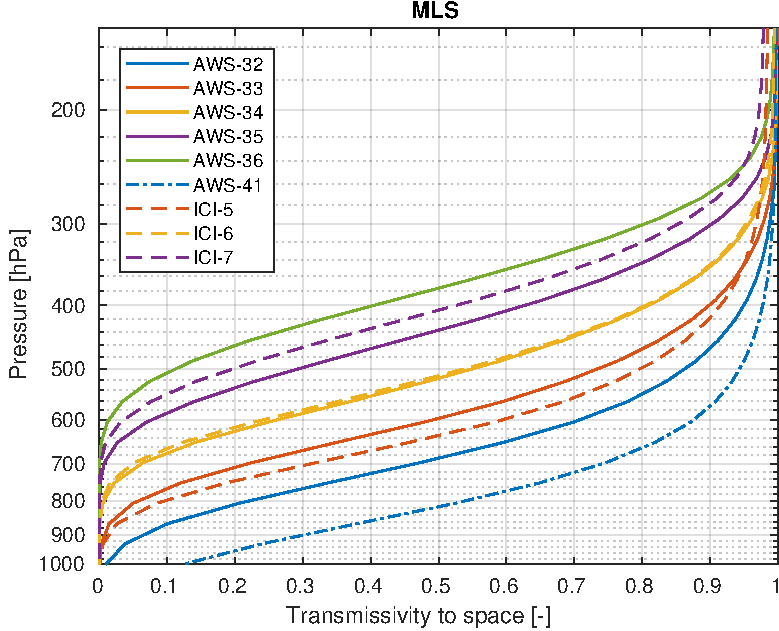
\includegraphics[width=0.75\textwidth]{fascod_tr_mls}
  \caption{Transmissivity to space as a function of altitude, for the
    mid-latitude summer scenario. Solid lines represent 183\,GHz channels,
    dashed lines 325\,GHz channels and dashed-dotted the 229\,GHz channel
    (Table~\ref{tab:fixed:chs}). These transmissivities are independent of
    surface reflectivity.}
  \label{fig:tr:mls}
\end{figure}
\begin{figure}[p]
  \centering
  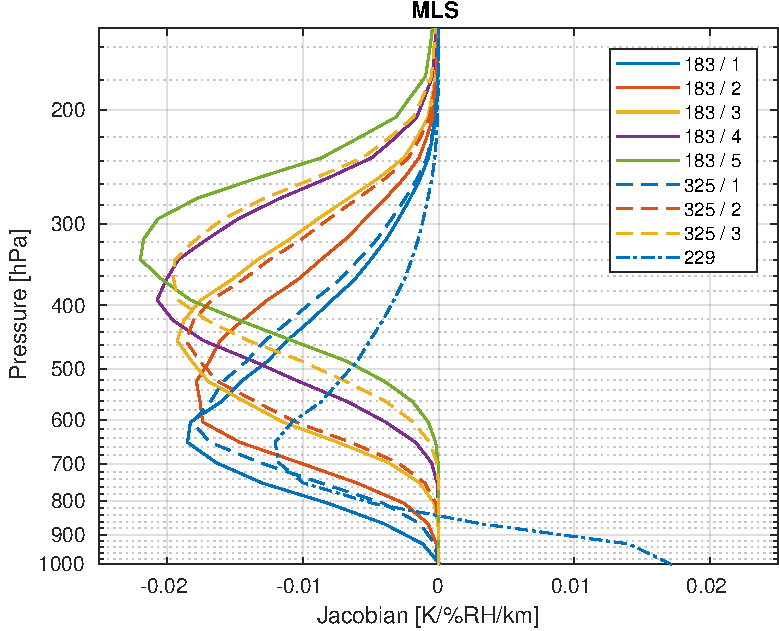
\includegraphics[width=0.75\textwidth]{fascod_wf_mls_025}
  \caption{Jacobians for relative humidity. Line symbols as in Fig.~\ref{fig:tr:mls}.
    Surface reflectivity is set to 0.25.}
  \label{fig:wf:mls:025}
\end{figure}

For 183 and 325\,GHz the brightness temperatures increase when moving away from
the centre frequency of the transition. The ``kinks'' in the spectra correspond
to ozone transitions, that are both more frequent and stronger in the 325\,GHz
range than in the 183\,GHz one. See Fig.~1 of \citet{eriksson:towar:20} for how
the ozone transitions are distributed between the lower and upper 325\,GHz
sideband. The spectra of 183 and 325\,GHz deviate little close to the transition
frequency, showing that the two frequencies are of similar strength, though the
325\,GHz one is slightly weaker. The higher deviations further out in the wings
are due to different contribution of far wing and continuum absorption, that is
higher at 325\,GHz. The 229\,GHz brightness temperatures are higher than any
value around 183 and 325\,GHz, as expected 229\,GHz being a window channel.

In Fig.~\ref{fig:tb:r050} the surface reflectivity is changed to 0.5, which
should roughly correspond to the highest reflectivity encountered at these
frequencies. The differences to Fig.~\ref{fig:tb:r000}  are small for 183 and
325\,GHz for the tropical and the two summer scenarios. On the other hand,
there is a clear impact in the wing part of 183\,GHz for the two winter
scenarios. The same is true for 325\,GHz, but the influence of the surface
reflectivity is considerably lower.  Beside for the tropical case, for
229\,GHz there is a pronounced dependency of the surface reflectivity, e.g.\
about 35\,K for mid-latitude winter.


\subsection{Clear-sky transmissivities to space}
%
Assuming that a cloud layer can be moved in altitude, its impact on measured
brightness temperatures will roughly follow the transmissivity to space for the
cloud altitude. In short, where the transmissivity is zero the cloud will have
no impact, while where the transmissivity is unity the influence will be close
to constant with altitude (especially when the single scattering albedo is
high). This relationship just refers to the relative impact for a
given frequency, the absolute impact (at transmissivity 1) increases in general
with frequency. 

Figure~\ref{fig:tr:mls} displays examples on transmissivities to space. The
transmissivities refers to the up-welling radiation. The contribution from
reflected down-welling is neglected and the considered transmissivity does not
depend on surface reflectivity.

The altitude variation of transmissivity exhibits same basic shape between all
the 183 and 325\,GHz channels, but the altitude of optical thickness of 1
(transmissivity of $e^{-1}\approx0.37$) varies. The curves of the edge 183\,GHz
channels (AWS-32 and 36) brackets the ones corresponding to the ICI 325\,GHZ
channels. The later channels show a higher deviation from 1 at 150\,hPa, due to
some (weak) ozone attenuation in the stratosphere. The 229\,GHz has the highest
transmissivities.


\subsection{Clear-sky relative humidity weighting functions}
%
The sensitivity to humidity is most easily compared by the channels' weighting
functions (i.e.\ the Jacobian), and examples are found in
Fig.~\ref{fig:wf:mls:025}. The shape of the weighting functions depends on the
unity selected for representing water vapour. As the absolute amount of water
vapour varies with orders of magnitude from the surface to the tropopause, it
is difficult to interpret weighting functions for absolute humidity units and
it is more suitable to use a relative one. In Fig.~\ref{fig:wf:mls:025} the
weighting functions correspond to an increase of relative humidity (RH) with one
percent unit over 1\,km. RH with respect liquid/ice is applied above/below
0$^\circ$C.

The basic shape of the Jacobian is similar for all 183 and 325\,GHz channels,
but the peak altitude varies. Again the edge 183\,GHz channels brackets the
325\,GHz ICI ones, as for transmissivity. These Jacobians are negative, meaning
that a change towards higher humidity results in decreased brightness
temperatures. The 229\,GHz Jacobian is positive close to the surface, as this
channel has sensitivity all the way down to the surface and more water vapour
just above a reflecting surface results in higher brightness temperatures. The
switch from negative to positive Jacobian depends on atmospheric scenario and
surface reflectivity. For dry conditions also the outer 183 and 325\,GHz
channels can have a positive part, as long as the reflectivity is not close to
0.


\section{Preliminary options for 325\,GHz channels}

[* Anders just informed us (May 29) that it would be good to avoid an IF of 1.7\,GHz, as that frequency could be used for downlink and there is a risk for
interference. The four channel option can easily be adopted to this, but what
do with the three channel one? *]


\subsection{Impact of upper end of IF band}
%
Figure~\ref{fig:wfuns:325ul} assumes that the channel placed at the high end of
the IF band is 3\,GHz wide (as for ICI, Table~\ref{tab:fixed:chs}), and shows
the RH weighting function if the outer channel ends at 11, 10, 9 or 8\,GHz. The
weighting functions for each sideband are here kept separated.


As expected, when the channel is moved away the centre frequency, the weighting
function moves downwards. However, moving the channel from 5\,-\,8\,GHz to
8\,-\,11\,GHz (in IF) results only a small shift, about 400 and 200\,m for the
lower and upper side, respectively. In terms of the resulting double sideband
channel the the shift would be 300\,m. Accordingly, there is little gain by
enforcing the IF range to go above 8\,GHz. As a rule of thumb, a higher ratio
between highest and lowest IF is more costly to implement. Albeit small, a
negative consequence of a 8\,-\,11\,GHz channel, compared to 5\,-\,8\,GHz, is
some asymmetry in the altitude response between lower and upper sideband. This
asymmetry is caused by higher continuum and far wing absorption on the upper
side.

In summary, the benefit of extending the IF band above 8\,GHz is small and
placing channels above 8\,GHz seems unnecessary considering the limited budget
and development time of AWS.

\begin{figure}[!p]
  \centering
  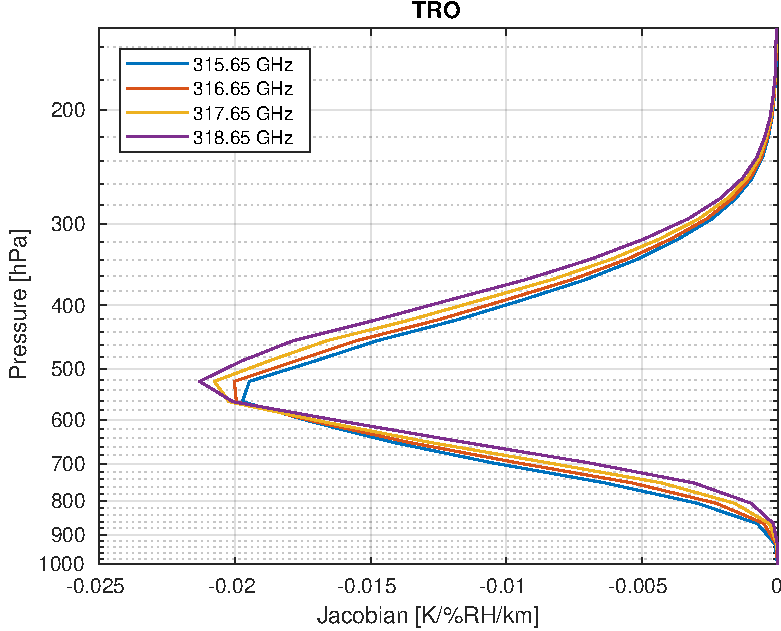
\includegraphics[height=61mm]{fascod_wf_325l_tro}\hspace{5mm}% 
  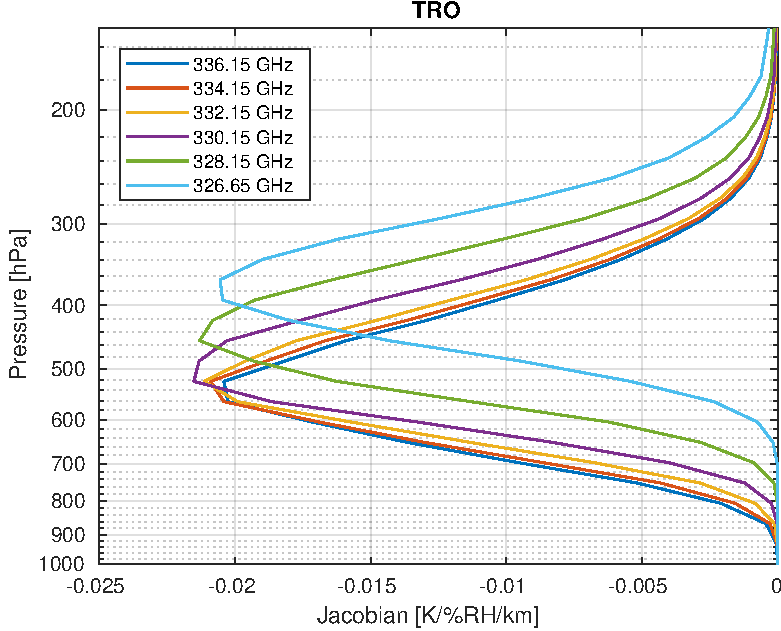
\includegraphics[clip,trim=43 0 0 0,height=61mm]{fascod_wf_325u_tro}
  \caption{RH weighting functions for the lower (left) and upper (right) side
    of the 325.15\,GHz transition. All weighting functions are for a 3\,GHz
    bandwidth. The stated frequencies are the centre frequency of each. In
    terms of IF range, the channels cover 8-11, 7-10, 6-9 and 5-8\,GHz (from
    top-to-bottom in the order given in the legends). }
  \label{fig:wfuns:325ul}
\end{figure}
\begin{figure}[!p]
  \centering
  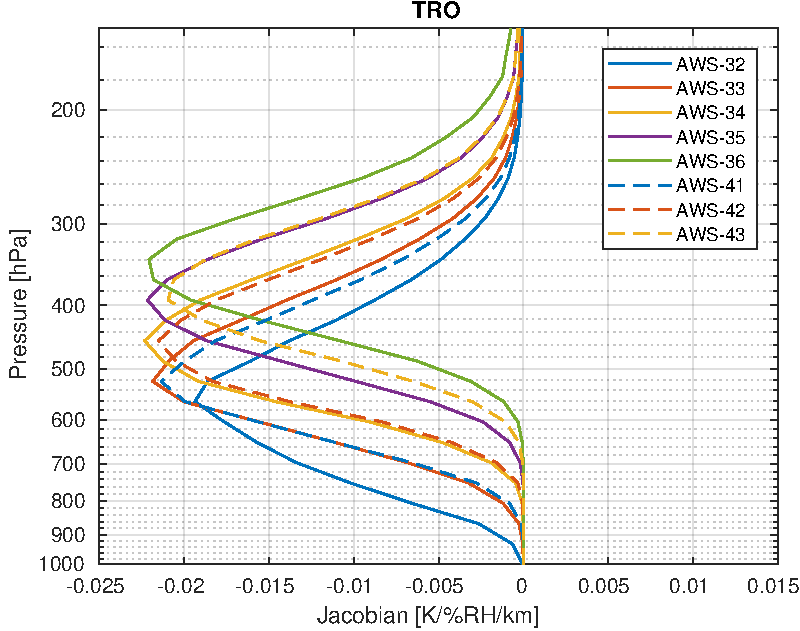
\includegraphics[height=61mm]{fascod_3chopt_tro}\hspace{5mm}% 
  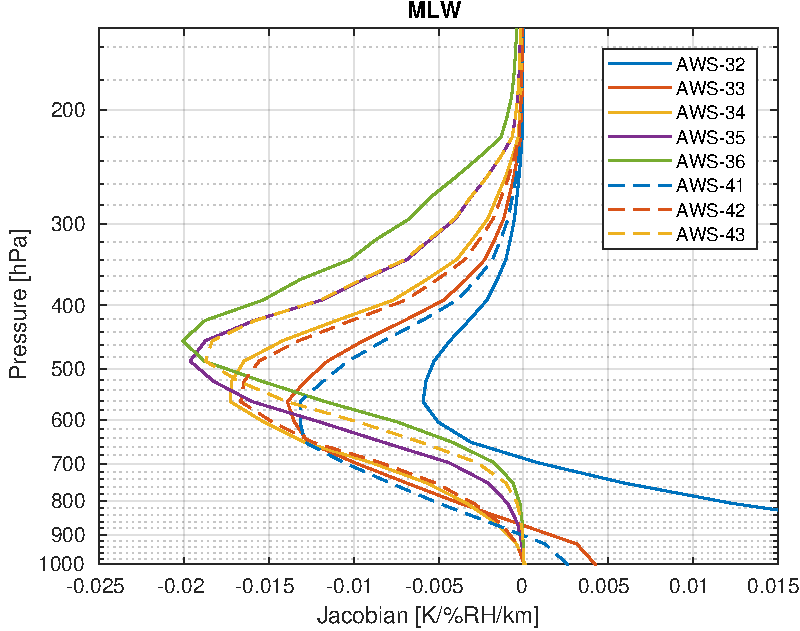
\includegraphics[clip,trim=43 0 0 0,height=61mm]{fascod_3chopt_mlw}
  \caption{RH weighting functions of the three channel option in
    Table~\ref{tab:chs:prel}, for the Fascod tropical (left) and mid-latitude
    winter (right) scenarios.}
  \label{fig:3ch:prel}
\end{figure}
\begin{figure}[!p]
  \centering
  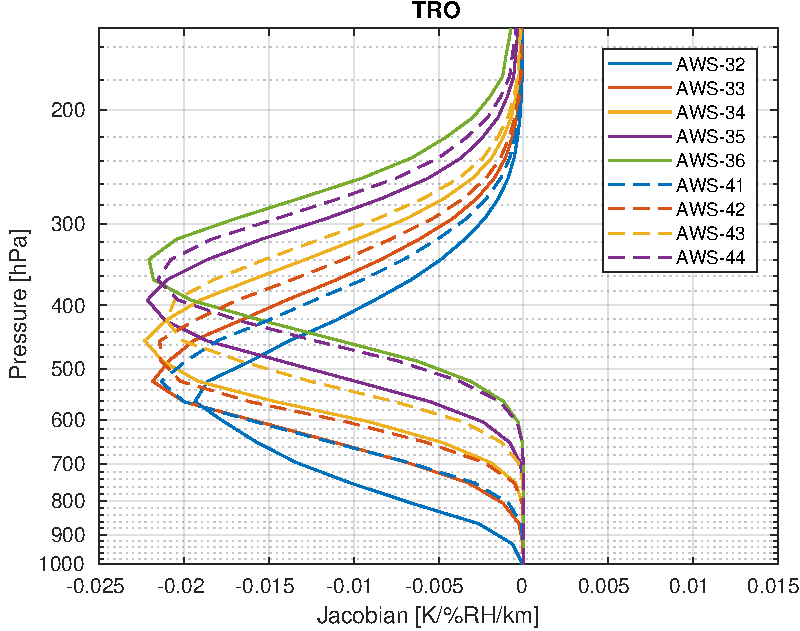
\includegraphics[height=61mm]{fascod_4chopt_tro}\hspace{5mm}% 
  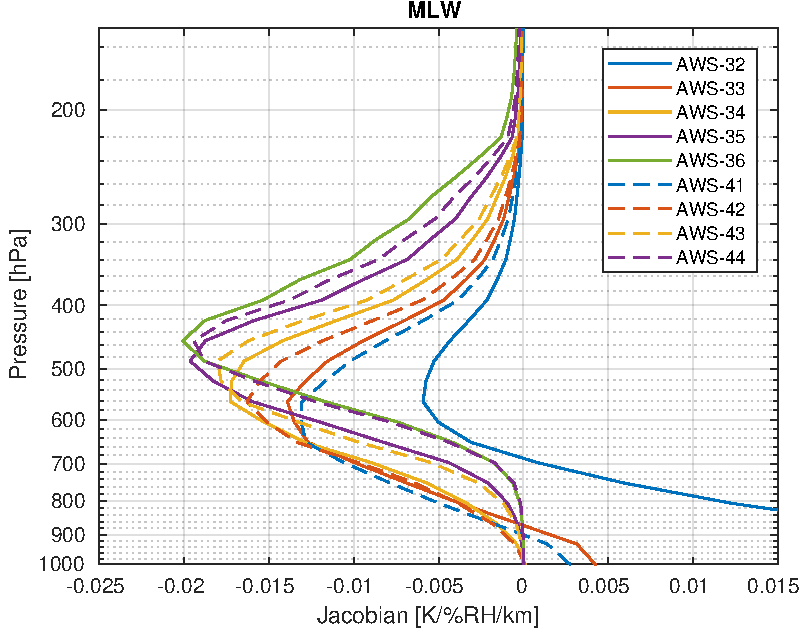
\includegraphics[clip,trim=43 0 0 0,height=61mm]{fascod_4chopt_mlw}
  \caption{RH weighting functions of the four channel option in
    Table~\ref{tab:chs:prel}, for the Fascod tropical (left) and mid-latitude
    winter (right) scenarios.}
  \label{fig:4ch:prel}
\end{figure}


\subsection{A three channel option}
%
The ICI channels give a rough RH weighting functions matching with AWS-32,
AWS-33 and AWS-34 (Fig.~\ref{fig:wf:mls:025}), and to find a tentative three
channel option an even better matching was used as constrain to set the
specifications. The resulting values are found in Table~\ref{tab:chs:prel} and
example weighting functions are displayed in Fig.~\ref {fig:3ch:prel}. This
option has a IF range of 1.0 to 8.0\,GHz, and leaves a 100\,MHz space between
AWS-42 and AWS-43, and 200\,MHz space between AWS-41 and AWS-42. That is, the
suggestion uses the complete IF bandwidth as far as possible, that is
technically possible.

\begin{table}[!t]
  \begin{minipage}[b]{0.5\linewidth}
  \centering  
  \begin{tabular}[c]{c|c|c}
    Channel & Frequency   & Bandwidth \\
    name    & [GHz] &  [MHz] \\
    \hline
    AWS-41  & 325.15$\pm$6.50 & 3000\\
    AWS-42  & 325.15$\pm$3.55 & 2500\\
    AWS-43  & 325.15$\pm$1.60 & 1200\\
    \hline
  \end{tabular}
  \end{minipage}%
  \begin{minipage}[b]{0.5\linewidth}
  \centering  
  \begin{tabular}[c]{c|c|c}
    Channel & Frequency   & Bandwidth \\
    name    & [GHz] &  [MHz] \\
    \hline
    AWS-41  & 325.15$\pm$6.60 & 2800\\
    AWS-42  & 325.15$\pm$4.05 & 1900\\
    AWS-43  & 325.15$\pm$2.35 & 1300\\
    AWS-44  & 325.15$\pm$1.20 & \phantom{0}800\\
    \hline
  \end{tabular}
  \end{minipage}  
  \caption{Preliminary specifications of AWS 325\,GHz channels, in the case of
    of three (left) and four (right) channels.}
  \label{tab:chs:prel}
\end{table}




\subsection{A four channel option}
%
The tentative four channel option in Table~\ref{tab:chs:prel} gives a broader
altitude coverage, towards higher altitudes, and offers weighting functions
roughly equally spaced in altitude (Fig.~\ref {fig:4ch:prel}). This option has
a IF range of 0.7 to 8.0\,GHz, and leaves 200\,MHz space between AWS-41 and
AWS-42 and has 100\,MHz between the other channels. Also this suggestion uses
the complete IF bandwidth.


\section{Cloud correction by a simple scheme}
\label{sec:simple}
%
In this section, the 325\,GHz three channel option is evaluated for detection
and correction of cloud interference in 183\,GHz channels. Combinations of
brightness temperature (TB) differences between 183\,GHz and 325\,GHz are used
as a measure of the cloud impact. A regression based approach is used to
estimate the adjustment needed to predict the clear-sky values.




\subsection{Formulation of correction scheme}
\label{sec:correction:scheme}
%
Let C1 and C2 represent one of the channels each from 183\,GHz and 325\,GHz,
respectively, and Tb1 and Tb2 represent the corresponding TB. The correction
scheme formulates a relationship between the cloud impact in C1 to the TB
differences between C1 and C2:
\begin{equation}
Tb1_{as}-Tb1_{cs} = f(x_m)
\label{eq:TB:diff}
\end{equation}
where, $x_m = Tb2_{as} - Tb1_{as}$, and the subscripts ``as'' and ``cs'' denote the all-sky and clear-sky cases respectively.  

The combinations of C1 and C2 are selected by matching their weighting
functions as shown in Fig.~\ref{fig:3ch:prel}. Five 183\,GHz and 325\,GHz paired
combinations are possible, for example one such paired combination is AWS-34
and AWS-42.

\begin{figure}[!tb]
	\centering
	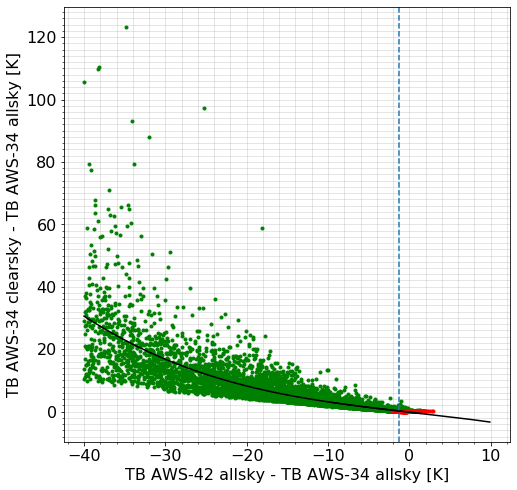
\includegraphics[height=85mm]{fit_AWS-34_AWS-42}\hspace{5mm}% 
	\caption{Brightness temperature difference of AWS-34 from AWS-42 plotted
      against cloud impact in AWS-34. Red and green colour represent the clear
      and cloudy cases respectively in the simulation dataset. The black curve
      represents the line of best fit (of green points) as a third order
      polynomial. The blue vertical line represents the correction threshold,
      $x_{cs}$, for $dtb_{cs} =$ 0.2\,K. }
	\label{fig:fit:c34-42}
\end{figure}
%

As an example, the relationship between the TB differences for C1 and C2 and
the cloud impact in C1 is shown in Fig.~\ref{fig:fit:c34-42}. For this
particular case, C1 is AWS-34 and C2 is AWS-42, and around 125\,000 simulations
are used. The two variables have a reasonably strong correlation for small TB
differences, but as the impact of cloud increases, the correlations gets
poorer. The data can be fitted by linear or non-linear models. The fitted model
can be used to obtain the adjustment required to compensate the brightness
temperature for cloudy cases. To avoid fitting the ``too cloudy'' cases which
do not show any reasonable correlation, cases with $Tb2-Tb1< -40$\,K are
excluded in the fit. Also, cases with a cloud impact below 0.2\,K (red colour
dots) can be considered as clear-sky, are not included in the model.

It is also important to have a manner for making a clear/cloudy classification
that can be derived from actual measurement data. This is useful for making
filtering in line with \citet{rekha2012potential}, but is also needed in the
correction scheme. The latter is the case as the polynomial fit derived gives a
non-zero correction for clear-sky cases. In Fig.~\ref{fig:fit:c34-42} the
difference between clear-sky values of channel C1 and C2 (red dots) have a mean
close to zero (as the weighting functions are well matched), but this is not
the case for all channel combinations and some general rule for finding a
threshold value (with respect to $x_m$) must be formulated. The polynomial fit
will be used also for this part.

We will simply treat cases that matches a correction below a certain value as
``clear-sky''. If the correction limit is denoted as $dtb_{cs}$, the threshold
value, $x_{cs}$, is obtained by inverting the polynomial fit:
\begin{equation}
x_{cs} = f_{cs}^{-1}(dtb_{cs}) 
\label{eq:dtb}
\end{equation}
That is, if $x_m>x_{cs}$ a measurement is classified as clear-sky. If
$x_m\leq x_{cs}$, the measurement is rejected if a pure filtering is made, or
it is adjusted if the correction scheme is applied. We will largely set
$dtb_{cs}$ based on the noise level of the 183\,GHz channel involved, to be
1$\sigma$ or 2$\sigma$ where $\sigma$ refers to the magnitude of measurement
noise (Eq.~\ref{eq:noise}, often called NE$\Delta$T). We will use $1\sigma$ for
the development of the scheme, however, the sensitivity of the scheme to
a 1$\sigma$ or 2$\sigma$ threshold is also provided later in the text.



\subsection{Application of correction scheme}
%
In this section, we test the applicability of the correction scheme in detail.
To analyse the performance of the approach, we apply it to correct the
measurements from C1 using data from C2. Without the availability of actual
data, the simulation dataset but with noise added is used mimic the measurements. The
noise for individual channels is calculated according to
Equation~\ref{eq:noise}. As an example, the results from the channel
combination AWS-34 and AWS-42 are shown. The error in the
predicted measurements is assessed as the deviation to corresponding noise-free
clear-sky value. The average bias, standard deviation and the measure of skewness, of the deviations are also calculated. Skewness gives a measure of asymmetry of the probability distribution of deviations around its mean.

To test the efficacy of the correction scheme, three different models: linear,
quadratic and cubic are evaluated to fit the TB differences between C1 and C2.
For all three models, cases with $Tb2-Tb1 < $ -15\,K are assumed to be ``too
cloudy'' and are not corrected. Also, cases classified as clear according to
the $1\sigma$ threshold are not corrected. The clear-sky adjustment for all
eligible measurements is calculated from all three models, and the three
predicted datasets are compared.

The occurrence frequency of the deviations from three models is shown in
Fig.~\ref{fig:correction:c34-42:fit} and their corresponding statistics are shown in Table~\ref{tab:correction:stats:34:42:allfits}. The occurrence frequency of the
measurements without any filtering or correction is also plotted as reference
(orange colour). If all measurements are devoid of cloud impact, the
deviations should follow the Gaussian distribution of noise. In such a case, the skewness of the deviations is close to zero.  However, in real conditions, the distribution has a large negative skewness due to the impact of clouds. After correction, all the three models are successful in reducing the cloud impact in the
measurements. The linear model has the lowest reduction in bias (from  -0.75\,K to -0.03\,K) but the highest values for skewness and standard deviation, in comparison to the other two models.  With the linear model, the error distribution of the corrected dataset has a relatively high positive skewness, which is undesirable. The positive skewness can be due to over-correction of cloudy cases, or erroneous correction of clear cases. The cubic  and quadratic models have almost similar statistics for bias and standard deviation, but the skewness in the cubic model is lower. Overall, the cubic model can be said to have the best performance, thus for all the results shown further, a cubic model is used.

In Sec.~\ref{sec:validation} the validation of simulations against ATMS data
(Fig.\ref{fig:pdf:c16-22}) showed that the cloudy cases in the simulations were
underrepresented in comparison to the observations. In order to have a higher
representation of cloudy cases, we thinned the measurement dataset by removing
50\% of the clear-sky cases. The distribution of thinned dataset is more closer
to real conditions in the region matching weak cloud impacts and all the
analyses presented further in this section are based on the thinned dataset.

Figure~\ref{fig:correction:c34-42:thinned} shows the deviation of the uncorrected and
corrected measurements to their noise-free clear-sky values for the thinned dataset. The results from
\cite{rekha2012potential} are also shown as reference (see Sec.~\ref{sec:rekha}
for our assumptions). In order to allow a more direct comparison of our
approach with \cite{rekha2012potential}, we also include the
dataset, ``Filtered'', where all cloudy cases are rejected. Apart from the fit
based cloudy classification, it is also assumed that cases with $Tb2-Tb1 < $
-15\,K are ``too-cloudy'' and are rejected.  To analyse the sensitivity of our scheme to noise threhold, as discussed in the previous section, results from two different values of $dtb_{cs}$ are shown. For both values of $dtb_{cs}$ the corresponding clear-sky cut-off
($x_{cs}$) is calculated using Eq~\ref{eq:dtb}. Various metrics corresponding to
the Figure~\ref{fig:correction:c34-42:thinned} are shown in
Table~\ref{tab:correction:stats:34:42:thinned}.


\begin{figure}[!tb]
	\centering
	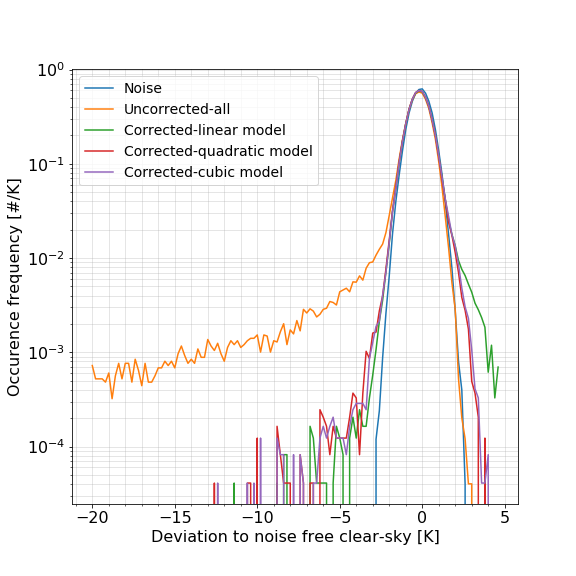
\includegraphics[height=85mm]{PDF_corrected_AWS-34_AWS-42_allfits}
	\caption{Deviation of AWS-34 measurements to noise free clear-sky
      simulations before and after correction, corrected using a linear,
      quadratic and cubic model. The distribution of noise alone is also shown
      as reference. The measurements have been corrected using brightness
      temperatures from AWS-42. The clear/cloudy classification is made with $dtb_{cs} = 1\sigma$ and also cases with $Tb2 - Tb1 > -15$\,K are rejected.}
	\label{fig:correction:c34-42:fit}
\end{figure}
%
\begin{table}[!tb]
	\centering
	\begin{tabular}[b]{c|c|c|c|c}
		Dataset  		  &   bias &   std &   skewness  & fraction  \\
		&   [K]  &   [K] & [-] & rejected [\%]\\
		\hline
		noise                     &   0.00 &  0.63 &               0.00 &                - \\
		uncorrected-all           &  -0.75 &  4.62 &             -11.78 &                - \\
		corrected-linear model    &  -0.03 &  0.75 &               0.48 &                2.84 \\
		corrected-quadratic model &  -0.06 &  0.71 &              -0.34 &                2.84 \\
		corrected-cubic model     &  -0.05 &  0.72 &              -0.23 &                2.84 \\
		\hline
	\end{tabular}
	\caption{Bias, standard deviation (std), and measure of skewness of error distributions
		shown in Figure~\ref{fig:correction:c34-42:fit}.The fraction rejected describes the percentage of cases which are removed. Results from three different fit models are shown: linear, quadratic and cubic.}
	\label{tab:correction:stats:34:42:allfits}
\end{table}
%
\begin{figure}[!tb]
	\centering
	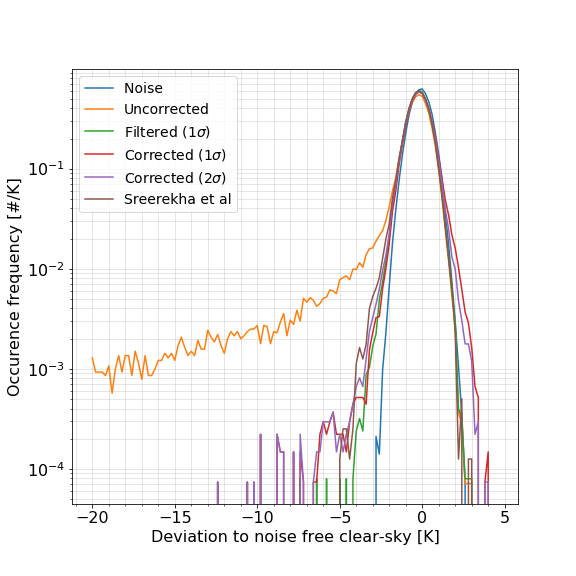
\includegraphics[height=85mm]{PDF_corrected_AWS-34_AWS-42_thinned}
	\caption{Deviation of AWS-34 measurements to noise free clear-sky
      simulations before and after correction. The measurements have been
      corrected using a cubic model. The different datasets are: noise
      (simulation dataset), uncorrected (thinned measurements), filtered $1\sigma$ (cases classified as cloudy according to $dtb_{cs}$ = 1$\sigma$ are rejected), corrected $1\sigma$ (cases classified as cloudy according to $dtb_{cs}$ = 1$\sigma$ are corrected), corrected
      $2\sigma$ (cases classified as cloudy according to $dtb_{cs}$ = 2$\sigma$ are corrected), Sreerekha et al (cloudy cases are filtered according to \citet{rekha2012potential}).}
	\label{fig:correction:c34-42:thinned}
\end{figure}
%
\begin{table}[!tb]
	\centering
	\begin{tabular}[b]{c|c|c|c|c}
		Dataset  		  &   bias &   std &   skewness  & fraction  \\
		&   [K]  &   [K] & [-] & rejected [\%]\\
		\hline
	noise             		&   0.00 &  0.63 &              -0.01 &                - \\
	uncorrected     		&  -1.27 &  6.05 &              -8.97 &                - \\
	filtered($1\sigma$)  	&  -0.13 &  0.68 &              -0.25 &               17.54 \\
	corrected($1\sigma$) 	&  -0.06 &  0.76 &              -0.46 &                4.99 \\
	corrected($2\sigma$) 	&  -0.11 &  0.75 &              -0.69 &                4.99 \\
	sreerekha et al   		&  -0.20 &  0.78 &              -1.00 &               45.36 \\			
		\hline
\end{tabular}
\caption{Bias, standard deviation (std), and measure of skewness of the
	error distributions of datasets shown in Figure~\ref{fig:correction:c34-42:thinned}.}
\label{tab:correction:stats:34:42:thinned}
\end{table}

The distributions of filtered data are non-Gaussian. The right side of the
distribution follows measurement noise while the left side is skewed. The
skewness in the distribution is due to cloud impacts which pass through the
clear-sky threshold. The higher skewness in ``Sreerekha et al'' is mainly
beacuse their method only aims at removing cloud impacts above 4\,K.
Their approach also leads to a high rejection fraction (45.36\%). The filtering
method introduced here leads to a considerable lower rejection of data
(17.54\%).

If the correction part for $1\sigma$ is added, the rejection is decreased even further (4.99\%)
and the bias is also improved (from -1.27 to -0.06\,K). On the other hand, the
correction gives some increase in standard deviation and skewness, compared to
filtering alone. A correction using $2\sigma$ gives poorer performance, in particular the reduction in bias is smaller and the skewness is increased.


%
\subsection{Application of correction scheme using AWS-4X}
%
\begin{figure}[!t]
	\centering
	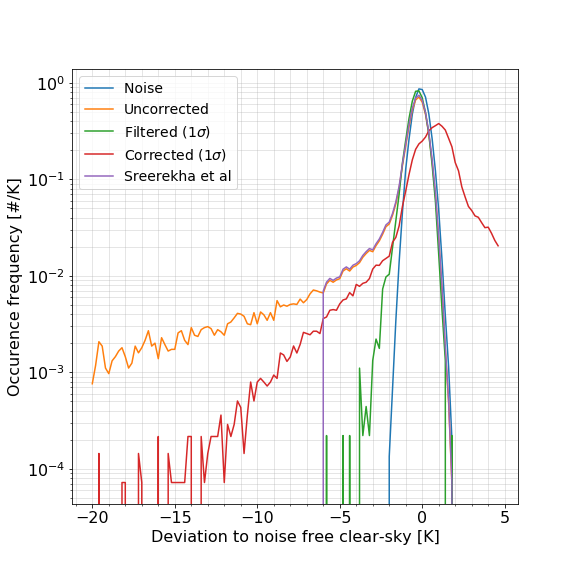
\includegraphics[height=85mm]{PDF_corrected_AWS-32_AWS-4X_thinned}
	\caption{Same as Fig.~\ref{fig:correction:c34-42:thinned}, but for channel combinations AWS-32 and AWS-4X. The dataset ``corrected 2$\sigma$'' is not shown.  }
	\label{fig:correction:c32-4X:thinned}
\end{figure}
%

As a reference with respect to having a channel at 229\,GHz, we also apply the
correction scheme described above to correct AWS-32 using AWS-4X (following
\citet{rekha2012potential}). In this case, C1 and C2 are AWS-32 and AWS-4X. The
TB correlations between AWS-32 and AWS-4X are poor and show a large spread
particularly for large cloud impacts (not shown). We fit the data to a polynomial model as described in Sec.~\ref{sec:correction:scheme} but exclude cases with $Tb2-Tb1 <$ -20\,K in the fit.

Fig.~\ref{fig:correction:c32-4X:thinned} shows the deviations of the
measurements to clear-sky values before and after correction, and the
corresponding metrics are provided in Table~\ref{tab:correction:stats:32:4X}.
With clear/cloudy classification for $dtb_{cs} = 1\sigma$, around 85\% of the
total measurements are classified as cloudy and are rejected in pure-filtering.
Rejecting all the cloudy cases reduces the average bias in the measurements
from -2.25\,K to -0.21\,K, while with the approach from
\citet{rekha2012potential} only 45.36\% of the data is rejected and the average
bias reduces to -0.41\,K. When all the cloudy cases, except the ``too cloudy'',
are corrected, the total bias increases to 0.88\,K. The unusually high fraction
of cloudy cases and an increase in bias on correction suggests misclassification
of clear cases as cloudy. Since, the weighting functions of AWS-32 and AWS-4X
are poorly matched, their relationship is inadequate to estimate the cloud
impact in AWS-32. Without any additional information, the regression approach
can only provide a successful filtering in comparison to the original approach
described by \citet{rekha2012potential}, although at the cost of high rejection
fraction. Additional information e.g., TB from other channels, is necessary
improve the accuracy of the correction.

\begin{table}[!h]
	\centering
	\begin{tabular}[b]{c|c|c|c|c}
		Dataset  		  &   bias &   std & skewness & fraction \\
						&   [K]  &   [K] & [-] 		& rejected [\%]\\
		\hline
Noise             		&  0.00 &  0.45 &               0.01 &                - \\
uncorrected       		&  -2.25 &  8.94 &              -6.85 &                - \\
filtered($1\sigma$)  	&  -0.21 &  0.51 &              -0.65 &               85.43 \\
corrected($1\sigma$) 	&   0.88 &  1.76 &              -1.30 &                5.35 \\
corrected($2\sigma$) 	&   0.76 &  1.80 &              -1.07 &                5.35 \\
sreerekha et al   		&  -0.41 &  1.00 &              -2.54 &               45.36 \\
		\hline
	\end{tabular}
	\caption{Same as Table~\ref{tab:correction:stats:34:42:thinned}, but for channel combinations: AWS-32 and AWS-4X.  }
	\label{tab:correction:stats:32:4X}
\end{table}

\subsection{Application of correction scheme to AWS-32, AWS-33, AWS-35 and AWS-36}
%
The correction scheme can also be extended to other combinations of 183GHz and
325GHz channels. The most relevant combinations for clear-sky screening are: AWS-32 and
AWS-41; AWS-33 and AWS-41; AWS-35 and AWS-43; AWS-36 and AWS-43.

Table~\ref{tab:correction:stats:32:41} shows the statistics when AWS-32 is
corrected using AWS-41. The statistics of the filtered dataset are better than
the approach by \cite{rekha2012potential}, while the corrected data have poorer
statistics. This is not surprising as the weighting function match between
AWS-32 and AWS-41 is poor. The correction using $2\sigma$ as threshold works
better $1\sigma$. This is an exception, the reverse is valid for AWS-34/42 (as
mentioned) and the channel combinations discussed below.

Table~\ref{tab:correction:stats:33:41} shows the statistics when AWS-33 is
corrected using AWS-41. The TB differences for this combination and the cloud
impact in AWS-33 are highly correlated. Rejecting the cloudy cases reduces the
average bias in the measurements from -1.74\,K to -0.13\,K, while a correction
of cloudy cases reduces the bias further to 0.05\,K. The standard deviation and
skewness of the corrected dataset are higher than pure-filtering, but smaller
than the approach by Sreerekha et al. Using $2\sigma$ threshold corrects a
smaller fraction of cases than $1\sigma$ but the overall statistics are poorer
in comparison to $1\sigma$, but still better than Sreerekha et al.

Table~\ref{tab:correction:stats:35:43} shows the statistics for the combination AWS-35 and AWS-43. Here the two filtered datasets have a comparable performance, while on correction, the bias is reduced, but skewness and standard deviation are increased. After correction ($1\sigma$) the bias due to cloudy measurements reduces from -0.83\,K to 0.01\,K while rejecting only 2.86\% of the total cases.  The performance of $1\sigma$ threshold in this case is also better than $2\sigma$.  
 
 
Table~\ref{tab:correction:stats:36:43} shows the statistics when AWS-36 is
corrected using AWS-43. For this combination, the weighting functions have a
poor match, but the TB differences and the cloud impact are strongly
correlated, as the cloud impact in AWS-36 is relatively low in comparison to
other 183\,GHz channels. The low fraction of rejection (7.38\%) also shows that
most of the measurements are without cloud impact. However, the small fraction
of cloudy cases which are corrected, helps in successfully reducing the average
bias from -0.54\,K to -0.07\,K.



\begin{table}[!p]
	\centering
	\begin{tabular}[b]{c|c|c|c|c}
		Dataset  		  &   bias &   std & skewness & fraction \\
							&   [K]  &   [K] & [-] & rejected [\%]\\
		\hline
noise             		&   0.00 &  0.45 &               0.00 &                - \\
uncorrected       		&  -2.25 &  8.94 &              -6.85 &                 - \\
filtered($1\sigma$)  	&  -0.26 &  0.77 &             -16.33 &               72.06 \\
corrected($1\sigma$) 	&   0.43 &  1.70 &             -14.68 &                7.93 \\
corrected($2\sigma$) 	&   0.25 &  1.72 &             -13.86 &                7.93 \\
sreerekha et al   		&  -0.41 &  1.00 &              -2.54 &               45.36 \\
\hline
	\end{tabular}
	\caption{Same as Table~\ref{tab:correction:stats:34:42:thinned}, but for channel combination: AWS-32 and AWS-41.   }
	\label{tab:correction:stats:32:41}
\end{table}

\begin{table}[!p]
	\centering
	\begin{tabular}[b]{c|c|c|c|c}
		Dataset  		  &   bias &   std &  skewness  & fraction\\
						&   [K]  &   [K] & [-]  & rejected [\%]\\
		\hline
	noise       	    	&  0.00 &  0.45 &               0.00 &               - \\
	uncorrected	    		&  -1.74 &  7.45 &              -7.77 &                - \\
	filtered($1\sigma$)  	&  -0.13 &  0.49 &              -0.40 &               26.18 \\
	corrected($1\sigma$) 	&  -0.05 &  0.59 &              -0.85 &                6.88 \\
	corrected($2\sigma$) 	&  -0.11 &  0.57 &              -1.17 &                6.88 \\
	sreerekha et al   		&  -0.29 &  0.78 &              -2.22 &               45.36 \\
		\hline
	\end{tabular}
	\caption{Same as Table~\ref{tab:correction:stats:34:42:thinned}, but for channel combination: AWS-33 and AWS-41.   }
	\label{tab:correction:stats:33:41}
\end{table}

\begin{table}[!p]
	\centering
	\begin{tabular}[b]{c|c|c|c|c}
		Dataset  		  &   bias &   std &   skewness & fraction \\
							&   [K]  &   [K] & [-] & rejected [\%]\\
		\hline
 Noise           	  &  0.00 &  0.63 &               0.00 &                -\\
uncorrected     	  &  -0.83 &  4.50 &             -10.85 &                - \\
filtered($1\sigma$)	  &  -0.13 &  0.68 &              -0.46 &               21.30 \\
corrected($1\sigma$)  &   0.01 &  0.90 &              -1.65 &                2.86 \\
corrected($2\sigma$)  &  -0.09 &  0.83 &              -2.35 &                2.86 \\
sreerekha et al  	  &  -0.13 &  0.70 &              -0.54 &               45.36 \\
		\hline
	\end{tabular}
	\caption{Same as Table~\ref{tab:correction:stats:34:42:thinned}, but for channel combination: AWS-35 and AWS-43.}
	\label{tab:correction:stats:35:43}
\end{table}

\begin{table}[!p]
	\centering
	\begin{tabular}[b]{c|c|c|c|c}
		Dataset  		  &   bias &   std &   skewness & fraction  \\
							&   [K]  &   [K] & [-] & rejected [\%]\\
		\hline
 Noise            	 &  0.00 &  0.88 &              -0.01 &               - \\
uncorrected      	 &  -0.54 &  3.40 &             -12.26 &                - \\
filtered($1\sigma$)  &  -0.11 &  0.92 &              -0.13 &                7.38 \\
corrected($1\sigma$) &  -0.07 &  0.93 &              -0.07 &                2.50 \\
corrected($2\sigma$) &  -0.11 &  0.94 &              -0.19 &                2.50 \\
sreerekha et al 	 &  -0.09 &  0.91 &              -0.10 &               45.36 \\
		\hline
	\end{tabular}
	\caption{Same as Table~\ref{tab:correction:stats:34:42:thinned}, but for channel combination: AWS-36 and AWS-43.   }
	\label{tab:correction:stats:36:43}
\end{table}


\section{Cloud correction by QRNN}
%
There are two main drawbacks of the simple scheme introdoced in the previous
section. The filtering/correction only involves a single 325\,GHz channel. The
scheme could be extended to consider a higher number of channels, but there is
no obvious formulation of the expressions to apply. The second problem is that
no case-specific uncertainty estimate is provided, only the overal bias and
standard deviations are known. The first drawback hints towards using a machine
learning approach, and the second one suggests to use the special form denoted
QRNN (Quantile Regression Neural Network), that was introduced for ratmospheric
retrievals by \citet{pfreundschuh:aneur:18}.

\dots


\section{Discussion}

\subsection{229 vs.\ 325\,GHz}


\subsubsection{Altitude coverage}
%
This discussion is based on figures and text found in Sec.~\ref{sec:overview}.
A basic remark is that a channel at 229\,GHz channel has a lower sounding
altitude than all the 183\,GHz channels for clear-sky conditions. Accordingly,
there are no matching RH weighting functions between 229\,GHz and 183\,GHz
channels. On the other hand, channels around 325\,GHz have quite similar
characteristics as some of the 183\,GHz channels (for clear-sky), but
consistently have a sounding altitude above the one of AWS-32.

With respect to sensitivity to hydrometeors, 229\,GHz will react on rain and
clouds at lower altitudes than the 183\,GHz channels. Due to the lower sounding
altitude, 229\,GHz is also more influenced by the surface. Both these aspects
could be beneficial in a wider perspective, but are not ideal for cloud
filtering of 183\,GHz data. With respect to this application, the main drawback
of the 325\,GHz region is the lack of a full coverage for AWS-32. There exists
an altitude range where hydrometeors have an impact on AWS-32 but will largely
be undetected by the 325\,GHz channels.


\subsubsection{Performance of the basic scheme}
%
A simple approach for cloud filtering/correction based on 325\,GHz data is
tested in Sec.~\ref{sec:simple}. The approach requires simulations for deriving
some parameters (in the form of a polynomial fit), while the application only
involves measurement data. Another advantage of the approach is that it is
channel specific. That is, it could result in that e.g.\ AWS-32 and 33 are
rejected, while that data for the higher peaking channels still can be used.

The results for AWS-33, 34, 35 and 36 should be considered as satisfactorily.
In short, a relatively low rejection rate is achieved and still data with
relatively narrow and symmetric error distributions are provided. The lowest
standard deviation and skewness are obtained by just performing a filtering.
Activating the correction part (with $1\sigma$ as threshold value) decreases
the bias and rejection rates significantly, but comes with the cost of
increased standard deviation and skewness. However, the increase in standard
deviation is throughout below 50\% (compared to the ideal case of that the
error distribution only consists of noise). 

For AWS-32, filtering based either AWS-4X or AWS-41 has a very high rejection rate, though the resulting dataset has low error. The high fraction of rejection can increase the probability of removing ``true'' clear cases. After correction, the error distributions are asymmetric and have large bias and standard deviation. Among the two combinations, the dataset corrected with AWS-41 has slightly better bias and standard deviation. As an exception to other 183\,GHz channels, the correction scheme for AWS-32 works better for $2\sigma$ threshold, as with a larger value of noise, relatively smaller number of cases are corrected. The effect of mismatch between weighting functions for AWS-32 and AWS-4X/41 is reflected in the performance of our correction scheme.

\subsubsection{Comparison to \citet{rekha2012potential}}
%
Results from \citet{rekha2012potential} has been used as reference, but the
comparison should only be considered as being qualitative. A more detailed
comparison is not possible as the selection of atmospheric cases is very
different between the studies. While in this study we aim to have a statistical
distribution as close as possible to real conditions, there is a strong focus on
cloudy conditions in the simulations used by \citet{rekha2012potential}. Our
translation of the performance reported in \citet{rekha2012potential} to our
conditions is found in Sec.~\ref{sec:rekha}.

The results of \citet{rekha2012potential} is better than ours for AWS-32, while for the other 183\,GHz channels better results are obtained by using 325\,GHz data. However, when only pure-filtering is considered, our scheme performs better for AWS-32, albeit with a high rejection rate. For all later channels of 183\,GHz,  we reject only a small fraction of cases in comparison to \citet{rekha2012potential}, but the corrected datasets have symmetric error distributions with lower bias, standard deviations. Only for AWS-35 and AWS-36, the standard deviation and skewness of the corrected dataset is higher. 

It should be noted that the approach of \citet{rekha2012potential} involves
simulations for every case, to obtain a ``background minus observation''
difference, while in this study a similar or better performance is obtained
from using measurement data alone. 


\subsection{Technical implementation}

\subsubsection{Shape of channel response functions}
%
The simulations have assumed rectangularly shaped response functions. This was
done for simplicity and shall in no way be taken as an indication on that this
shape is required.

We have left some frequency gaps between the channels to simplify the technical
implementation, i.e.\ to decrease the demand on very sharp transitions from high
to low response. We have assumed that 100\,MHz is sufficient in the lower end
of the IF-range and 200\,MHz in the upper part. If found necessary we don't see
any problem in increasing the gaps, beside that the bandwidth decreases and the
NE$\Delta$T of the channel will somewhat increase.


\subsubsection{Polarisation response}
%
Polarisation aspects have not been considered in full detail. Some polarisation
is induced by the surface in the simulations, but hydrometeors are assumed to
be totally randomly oriented and do not cause polarisation. To involve oriented
particles was not possible due to the limited time allocated for the study.

The basic recommendation would be to use the same polarisation response as far
as possible. If both quasi-horizontal and quasi-vertical bands must be applied,
the recommendation prioritise to use the polarisation option for 183 and
325\,GHz, to maintain a similar influence of polarisation between the bands.







\section{Conclusion}
%
This study compares the options of having a channel at 229\,GHz or having some
around 325\,GHz from a single perspective, cloud filtering/correction of
183\,GHz data. There could be other important reasons to consider for the
selection.

\dots


{\footnotesize
\bibliography{j_abbr,references}
}

\end{document}
